
\documentclass{vldb}
\usepackage{balance}  
\usepackage{graphicx} 
\usepackage[hyphens]{url}      
\usepackage{amsmath}
\usepackage{color}
\usepackage{cancel}
\usepackage{listings}
\usepackage[normalem]{ulem}
\usepackage{graphicx}
\usepackage{subcaption}
\setlength{\abovecaptionskip}{10pt plus 3pt minus 2pt}
\usepackage{booktabs}
\usepackage{graphicx}
\usepackage[ruled,vlined,algonl,boxed]{algorithm2e}
\usepackage{algorithmic}
\usepackage{wrapfig}
\usepackage{enumitem}
\usepackage{xspace}
\usepackage{xcolor}
\usepackage{colortbl}
\usepackage[T1]{fontenc}
\usepackage{fancyvrb}
\usepackage[bottom]{footmisc}



\usepackage[nocompress]{cite}
\usepackage{microtype}
\usepackage[section]{placeins}

\makeatletter
\def\url@leostyle{
  \@ifundefined{selectfont}{\def\UrlFont{\sf}}{\def\UrlFont{\small\bf\ttfamily}}}
\makeatother
\urlstyle{leo}

\makeatletter
\def\@copyrightspace{\relax}
\makeatother

\def\pprw{8.5in}
\def\pprh{11in}
\special{papersize=\pprw,\pprh}
\setlength{\paperwidth}{\pprw}
\setlength{\paperheight}{\pprh}
\setlength{\pdfpagewidth}{\pprw}
\setlength{\pdfpageheight}{\pprh}

\newtheorem{definition}{Definition}
\newtheorem{proposition}[definition]{Proposition}
\newtheorem{lemma}[definition]{Lemma}
\newtheorem{remark}[definition]{Remark}
\newtheorem{corollary}[definition]{Corollary}
\newtheorem{claim}[definition]{Claim}
\newtheorem{theorem}[definition]{Theorem}
\newtheorem{heuristic}[definition]{Heuristic}
\newtheorem{example}[definition]{Example}
\newtheorem{dimension}{Dimension}
\newcounter{prob}
\newtheorem{problem}[prob]{Problem}
\newtheorem{conjecture}[definition]{Conjecture}
\newtheorem{reduction}[definition]{Reduction}
\newtheorem{property}[definition]{Property}
\newtheorem{axiom}[definition]{Axiom}











\usepackage[pdftex]{hyperref}
\hypersetup{
  colorlinks=false,
  linkcolor=darkred,
  citecolor=darkgreen,
  urlcolor=darkblue
}



\widowpenalty=10000
\clubpenalty=10000


\definecolor{light-gray}{gray}{0.95}
\definecolor{mid-gray}{gray}{0.85}
\definecolor{darkred}{rgb}{0.7,0.25,0.25}
\definecolor{darkgreen}{rgb}{0.15,0.55,0.15}
\definecolor{darkblue}{rgb}{0.1,0.1,0.5}
\definecolor{blue}{rgb}{0.19,0.58,1}

\newcommand{\red}[1]{\textcolor{red}{#1}}
\newcommand{\green}[1]{\textcolor{green}{#1}}
\newcommand{\blue}[1]{\textcolor{blue}{#1}}
\newcommand{\orange}[1]{\textcolor{orange}{#1}}
\newcommand{\darkred}[1]{\textcolor{darkred}{#1}}
\newcommand{\darkgreen}[1]{\textcolor{darkgreen}{#1}}
\newcommand{\darkblue}[1]{\textcolor{darkblue}{#1}}

\makeatletter
\setlength{\@fptop}{0pt}
\makeatother



\widowpenalty 10000
\clubpenalty 10000


\newcommand{\ind}{\hspace{\algorithmicindent}}

\newcommand{\deprecate}[1]{\noindent{\color{light-gray}{#1}}}



\pagenumbering{arabic}

\makeatletter
\def\maketag@@@#1{\hbox{\m@th\normalfont\normalsize#1}}
\DeclareRobustCommand*\textsubscript[1]{
          \@textsubscript{\selectfont#1}}
        \def\@textsubscript#1{
          {\m@th\ensuremath{_{\mbox{\fontsize\sf@size\z@#1}}}}}
\makeatother

\newcommand{\papertext}[1]{#1}
\newcommand{\techreport}[1]{#1}


\newcommand{\alex}[1]{\noindent{\color{darkgreen}{[Alexandra: #1]}}}
\newcommand{\xlw}[1]{\noindent{\color{blue}{Xiaolan: #1}}}
\newcommand{\ewu}[1]{\noindent{\color{red}{EWu: #1}}}

\newcommand{\xxx}[1]{{\fontsize{13pt}{13pt}\selectfont\textcolor{red}{#1}}}
\newcommand{\codesize}{\fontsize{7}{8}}
\newcommand{\stitle}[1]{\vspace{0.5em}\noindent\textbf{#1}}
\newcommand{\calF}[0]{$\cal{F}$}

\newcommand{\sys}{VISTREAM\xspace}
\newcommand{\heurstic}{\textsc{HEURISTIC}\xspace}

\setlength\floatsep{0.8\baselineskip plus 3pt minus 2pt}
\setlength\textfloatsep{0.9\baselineskip plus 3pt minus 2pt}
\setlength\intextsep{1\baselineskip plus 3pt minus 2 pt}


\begin{document}

\title{\sys: A Prefetching Viz System That Works}

 
% \numberofauthors{1}
%  \author{
%   \alignauthor Eugene Wu\\
%     \affaddr{Computer Science}\\
%     \affaddr{Columbia University}\\
%     \email{ewu@cs.columbia.edu}\\
% }




\maketitle

\begin{abstract}
    \looseness -1
\ewu{The text is unedited for style.  It focuses on argument structure:}

It is important to make visual data exploration interactive, meaning that the system visually responds to user inputs within $100$ milliseconds.
Although the db and viz communities are seeking to do this through faster query, networking and rendering techniques,
prediction has been argued as a promising approach---if we are able to predict what the user will request, then the results can be pre-computed so that they are ready.
This can speed up user exploration as well as the visualization's initial loading time---the ``loading dataset'' progress bar is commonplace.
Such approaches rely on accurate predictive models, and existing approaches tend to limit the set of allowed user operations (e.g., to panning and zooming operations) so that the prediction space is small enough that high quality models are possible.  
Thus, the number of allowed interactions is typically significantly smaller (e.g., 1-5) as compared to the allowed interactions in real visualization systems.
Unfortunately, it's unlikely that such models will work if allow dozens of possible interactions.

We use a simple model to understand the design space and find \xxx{something interesting including a design sweet spot}.
Based on the model we design a new system, \sys, that exploits this sweet spot by using three tricks:
1) high quality prediction independent of the number of allowed operations.
2) a streaming oriented system where, in contrast to a request-response model of communication, the client periodically sends distributions
of future operations based on our high quality predictor, and the server continuously sends a stream of data to the client's circular buffer.
3) explicitly leverage progressive encodings to \xxx{something smart}.
In our experiments on XXX, we find that the unique combination of all three tricks are necessary, and
can improve responsiveness by XXX at the $95^{th}$ percentile, and YYY maximum response time.
\end{abstract}

%!TEX root = ../main.tex

\section{Introduction}

\label{s:intro}

A number of design principles are emerging in terms of system architectures
for visual data exploration.

Classic1: in database (tioga, data splash)

Classic2: vis does everything.  If viz is super powerful, then it works, however data is large so may be infeasible.

Classic3: client server.  assumption that working set fits in the client.  elegant.  however speed is not its strong suit.
Despite recent work on declarative ned-to-end specification and a unified execution framework, rather than separate client and server systems, the fundamental hardware architecture of a thin client (e.g., browser, laptop) and resource rich server (e.g., database server, cloud) is a reality.

Techniques: faster DB.  
approximation pushed by vis and database folks -- key is progressive and measuring good enough.

However a bottleneck is the request-response model of interaction.    Despite fast, or even precomputed results, computing delays, networking hiccups, data transfer, client costs, and other factors can all affect the response times.

Prefetching has been the primary technique, because it can pipeline user decision making with request handling.  However the results from prior work has suggested an inherent trade-off between the numbero of available interactions in the interface and the effectiveness of prefetching.

Is a prefetching-oriented architecture feasible for rich interactive interfaces?  What are the design considerations to make such an approach realistic?  And what might such an architecture look like?

To answer this question, we used a simple model-based analysis of end-to-end latency to understand the prediction accuracies that are necessary under different concurrent request, approximation, and request latency regimes.  We find that, under concurrency=5, partial result of 25\%, and an aggressive target perceived latency threshold of 100, the prediction model needs 

Based on these observations, we have designed \sys, a streaming-based architecture that generalizes the request-response model to support rich interactive visual exploration interfaces.  The primary idea is to model user interactions as a series of probability distributions over possible visualization requests at a future time steps.  Under this model, a given request is simply an impulse distribution centered around the user's interaction, however by sending a distribution.  This is similar to the notion of a QueryIntent~\cite{ebenstein2016fluxquery} however used in this context not to predict what the user will do but for prefetching.


We combine this with a streaming push-based architecture where.

Progressive encoding enables.

Our current system assume precomputed data structures, future work includes online query processing costs.

This architecture is a novel combination of three necessary design decisions: an interface agnostic prediction model, a streaming architecture, and progressive visualizations.  Each in isolation is not enough.   This architecture supports interactive visualizations where requests can be modeled as SQL queries, including DVMS, Vega, Forecache, Tableau, and common data viz systems.

To summarize our contributions:

\begin{itemize}[leftmargin=*, topsep=0mm, itemsep=0mm]

\item We formally analyze the design space for prefetching-based visual data exploration systems to understand the conditions for which prefetching will be effective.

\item We design a novel client-server architecture.

\item We present a suite of optimizations that further reduce interaction response times, and show how to extend to new offline data structures, including sampling and data cubes.

\item We perform a thorough evaluation of the XXX characteristics \sys's performance.  

\end{itemize}


\section{Model-based Analysis}

As described in the introduction, prefetching has the potential to enable visualization systems to respond with interactive latencies.  However, current approaches are designed for interfaces with limited options for user interaction~\cite{}; many have suggested that increasing the expressivity of the interface (e.g., the number of possible user actions) makes the prediction task significantly more challenging.  In this section, we seek to understand the minimum accuracy for model needs in order to support low user perceived latencies, as well as the conditions that affect this accuracy.

\subsection{The Model}

Our goal is to estimate the minimum prediction accuracy $\alpha$ needed in order to ensure that the user perceived latency $l_{user}$ is below a fixed threshold (e.g. 100ms~\cite{} or 500ms).
Let $T=0$ be the time.
We assume that the user will perform her request at $T=t$ where $t \ge 0$, and that the cost of answering a request consists of fetching and rendering the results.
$l_{user}$ is defined as the time between $t$ and the change reflected in the visualization. 
Let $l_{net}$ be the latency to execute a request, transfer the results across the network, and render it on screen.   In a typical system, $l_{user} = l_{net}$, which can be undesirable when query processing or the network latency are high.
Prefetching allows the client to proactively answer a request at $T=0$ and store the results in a client cache.
If a future request accessed data in the cache, then it can take much less time $l_{cache} < l_{net}$ and result in a more responsive user perceived experience.

We now model the expected user perceived latency as $l_{cache} + max(0, l_{net} - t)$ if model accurately predicted the request, and $l_{net}$ if it mispredicted.  The $max()$ operation accounts for cases when the cost of a cache miss is larger than $t$:
$$l_{user} = (l_{cache} + max(0, l_{net}-t))\times \alpha + l_{net}\times(1-\alpha) $$
Rearranging the terms, we can derive the minimum prediction accuracy in order to maintain $l_{user}$.
%$$\alpha = \frac{l_{net} - l_{user}}{l_{net} - l_{cache}}$$
$$\alpha = \frac{l_{user} - l_{net}}{l_{cache} + max(0, l_{net}-t) - l_{net}}$$

Prior perception and interactive visualization literature have used both $100$ and $500$ millisecond response times as thresholds for what is considered interactive~\cite{liu2014effects}.   Similarly, we assume request latencies can vary from $0$ to $2$ seconds~\cite{}, which embodies latencies that stem from query processing, serialization, network latencies and client overheads.  Finally, it is typically challenging to make accurate predictions more than several hundred milliseconds into the future~\cite{pasqual2014mouse}; we vary the ratio $\frac{t}{l_{net}}$ between $0.5$ and $1$.   We use the above constants in our analysis below.

Figure~\ref{fig:model_base} plots the model accuracy for two commonly cited $l_{user}$ thresholds (100 and 500ms).  The x-axis varies $l_{net}$ and each line represents the percentage of the prefetching costs that the user will experience.  For instance, when $\frac{t}{l_{net}}=1$, the user initiates the request at $T=t=l_{net}$ and does not experience any of the prefetching costs, whereas when $\frac{t}{l_{net}}=0.5$, the prefetching request is only half complete by the time the user initiates her request at $T=0.5\times l_{net}$.  We use a vertical line to mark the network latency at $1$ second.  

The first observation is that when $l_{net}$ is smaller than the threshold, the user perceived accuracy is independent of the model accuracy.  When the threshold is $100$, the minimum model accuracy quickly exceeds $80\%$ by even a request latency of $500$ms; although the minimum accuracy is lower under the $500$ms threshold, the accuracy converges to $70\%$.
It is challenging to guarantee such high user prediction accuracy for a single request---the accuracy in existing literature is slightly above $50\%$ for a constrained user interface with 9 interaction options~\cite{battle2016dynamic}.

\ewu{Argue that assuming $t < l_{net}$ is a reasonable assumption.}

\begin{figure}[ht]
	\centering
	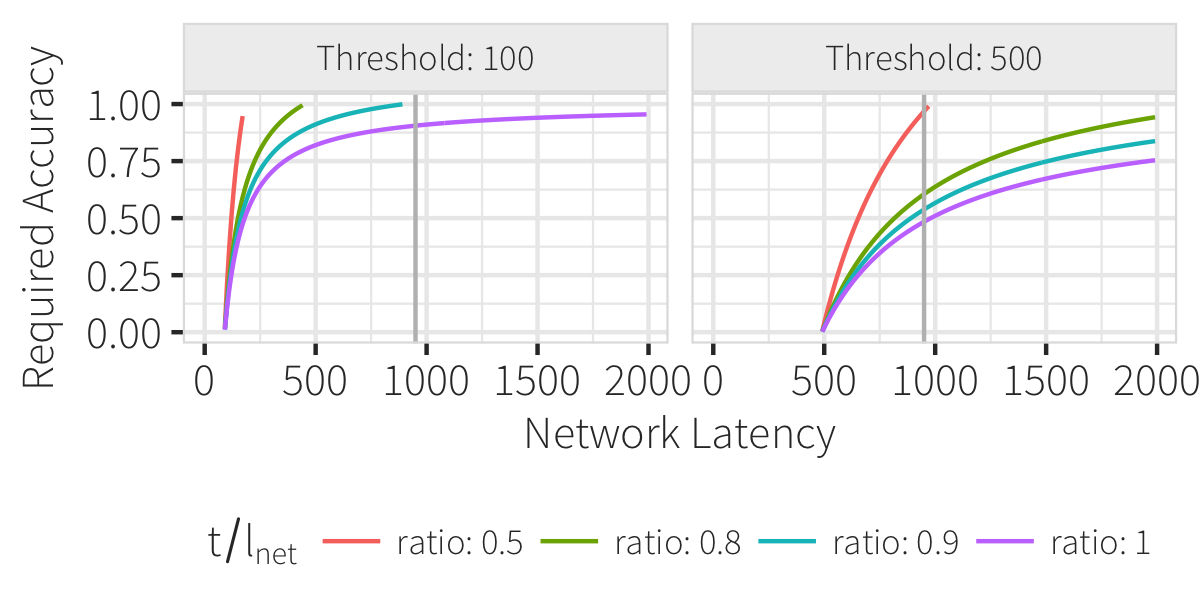
\includegraphics[width=1\columnwidth]{figures/model_base}
 	\caption{Minimum $\alpha$ vs network latency (x-axis), $\frac{t}{l_{net}}$ ratios (lines), and two thresholds (facets).}
    \label{fig:model_base}
\end{figure}



\stitle{Vary Prefetch Concurrency}
Most modern data processing systems are able to execute multiple concurrent requests~\cite{ebenstein2016fluxquery,giannikis2012shareddb}, thus we now modify the model to vary the number of concurrent prefetch requests $N$.
The $(1-\alpha)^N$ term is the probability that none of the prefetch requests match the user's actual request at $T=t$:
%
$$l_{user} = (l_{cache} + max(0, l_{net} - t)\times (1-(1-\alpha)^N) + l_{net}\times(1-\alpha)^N $$
%
Rearranging the terms results in the following minimum prediction accuracy:
%
$$\alpha = 1 - \left(\frac{l_{cache}+max(0,l_{net}-t)-l_{user}}{max(0,l_{net}-t)-l_{net}}\right)^{1/N}$$

\begin{figure}[h]
	\centering
	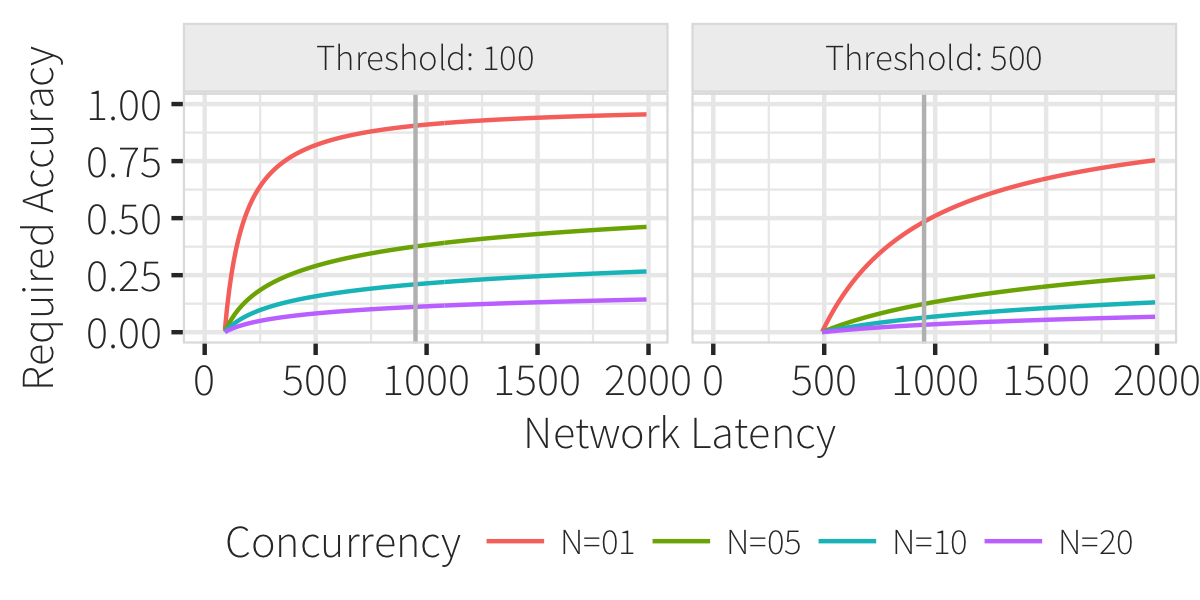
\includegraphics[width=1\columnwidth]{figures/model_concurrency}
 	\caption{Minimum $\alpha$ vs network latency (x-axis), concurrency (lines), and two latency thresholds (facets).}
  \label{fig:model_concurrency}
\end{figure}


Figure~\ref{fig:model_concurrency} shows that increasing the number of concurrent requests has an immediate effect on $\alpha$ ($t=l_{net}$ in these plots).    With $N=20$, a prediction model need only be $12\%$ accurate to ensure an interactive latency of $l_{user}=100$, while ensuring  $l_{user}=500$ only requires an accuracy of $3.5\%$.  At the limit, sending concurrent requests for all possible queries (assuming the cost is $l_{net}$) means the user latency is independent of prediction accuracy.  These results suggest that increasing the concurrency is an effective counter balance to model accuracy.


\stitle{Network Latency Variance}
Figure~\ref{fig:model_std} simulates $l_{net}$ drawn from a gaussian distribution with standard deviation of $std \in \{0, 100, 500\}$ milliseconds.  We set $N=20$, $t=l_{net}$, and the y-axis is from 0 to $0.4$.  Although the request variance affects the required model accuracy when $l_{net}$ is low, the curves for each threshold converge to the same levels independent of $std$; this is simply because $l_{net}$, rather than $std$, is the dominant factor as it increases.

\begin{figure}[h]
	\centering
	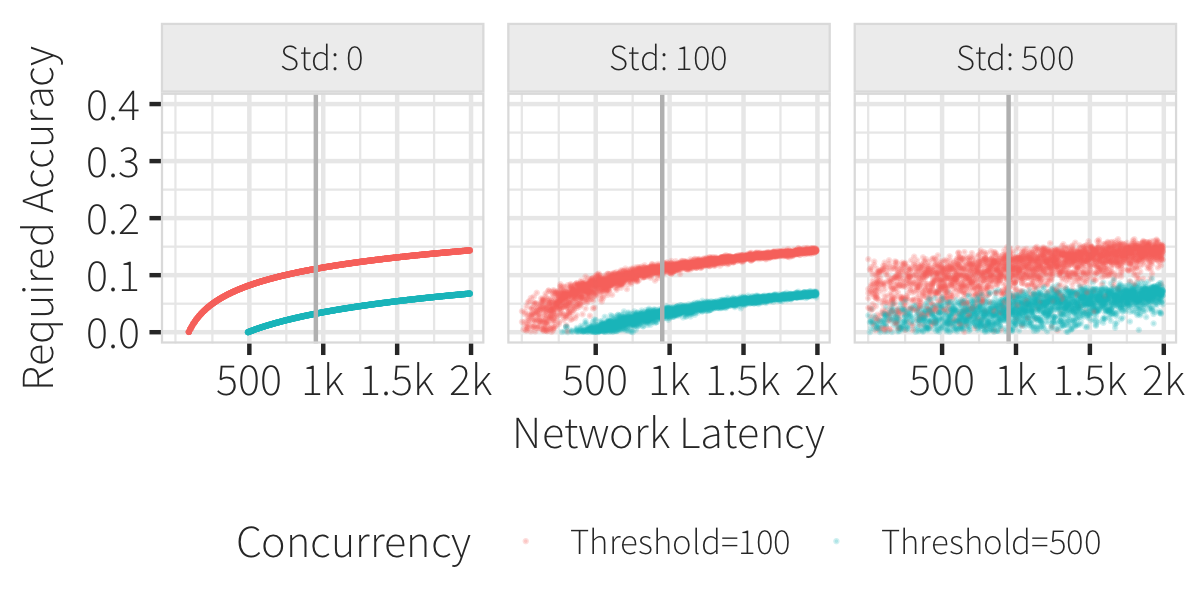
\includegraphics[width=1\columnwidth]{figures/model_std}
 	\caption{Minimum $\alpha$ vs network latency (x-axis), concurrency (lines), and two latency thresholds (facets).}
  \label{fig:model_std}
\end{figure}

\begin{figure}[h]
	\centering
	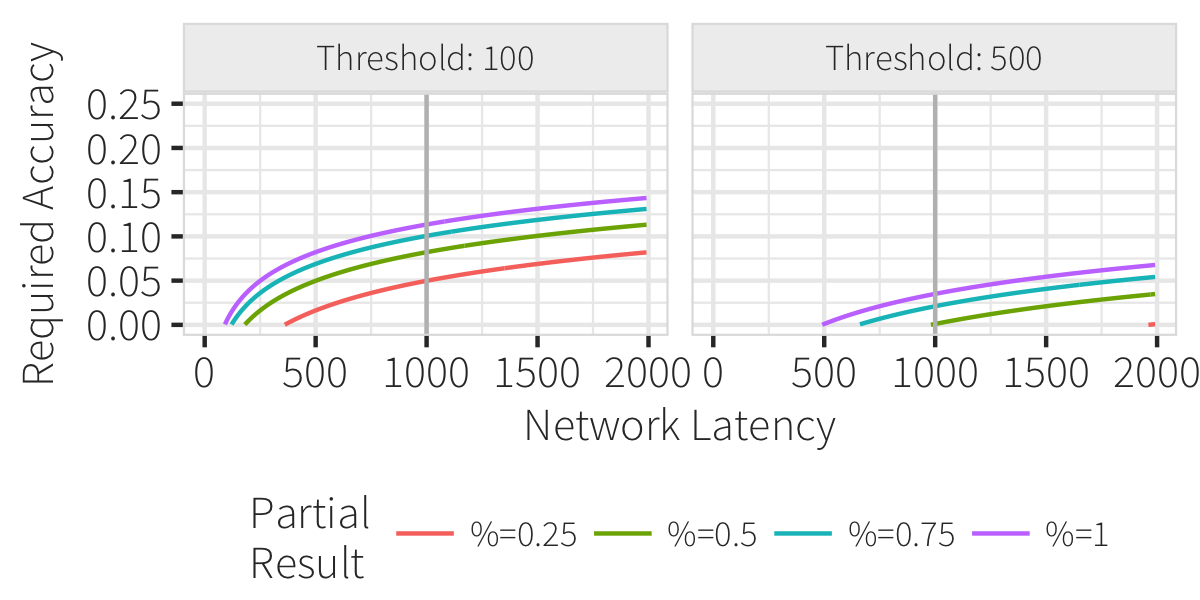
\includegraphics[width=1\columnwidth]{figures/model_partial}
 	\caption{Required prediction accuracy as a function of network latency, under progressive conditions where partial responses are sufficient.}
    \label{fig:model_partial}
\end{figure}


\stitle{Progressive Results}
The visualization and database communities have argued for approximate visualizations that are slightly inaccurate but potentially much faster to compute.  Techniques such as Online Aggergation~\cite{control,wanderjoin} or streaming wavelet compression~\cite{} are considered {\it progressive} because they are able to immediately return (and render) approximate results that improve over time; thus providing a natural trade-off between latency and result quality.  Our final analysis studies progressive results that require a fraction of the full request latency to be ``sufficiently good''.
\ewu{Use sampling and immens arguments as basis for 25\% partial results.} We find that $5\%$ accuracy is enough to maintain user perceived latency of $100$ when $25\%$ of the results is sufficient; at threshold of $500$, the perceived latency is independent of the model accuracy when $l_{net}\le 2000$.






\subsection{Discussion}
We find that a careful combination of existing techniques (concurrency and progressive results) can dramatically reduce the required model accuracy to enable low user perceived latency---in some extreme cases when the threshold is $500$, the model accuracy can even be $0\%$.  
\ewu{Argue that given  fixed network throughput between client and server, increasing concurrency beyond a certain point naturally requires partial results.  Thus the two go hand in hand.   We also see that the prediction model simply needs to be ``good enough'' with an accuracy of $5-10\%$.  When the number of possible interactions are limited to $10-20$ possible interactions, then even a random model is sufficient.  However in rich interfaces with potentially dozens or a hundred possible interactions, there may simply be too many choices to learn a good model.}


%!TEX root = ../main.tex


\section{Experiments}
\label{sec:experiments}

We run a series of micro and end-to-end system experiments to understand the performance improvements that each component contributes, as well as a user study to measure user-perceived latency.  These experiments use three different interactive visualization front-end designs that vary in the number of possible interactions that the user can perform---a simple pan-and-zoom map interface~\cite{}, a complex cross-filtering application, and an interface that is button-heavy.



\subsection{Experimental Setup}
This subsection describes our experimental setup and metrics.

\stitle{Traces: }
In our system experiments, we use \ewu{XXX} user traces collected from a Chromium extension running on the authors' browsers.  These traces were collected over the span of \ewu{XXX} weeks for all webpages that the authors browser.  The trace tracks mouse events (e.g., click, move, drag), as well as the type of page element that the user interacted with. 

We also collected a specialized set of user traces when interacting with custom interactive visualizations used in the user study, and labeled the type of interaction (e.g., button click, slider drag, pan, zoom in, etc).  For the visualization-based traces, we also logged the corresponding query requests for each mouse event in order to collect the ground truth.  The traces, visualizations, and queries will be released after publication.

To summarize, our traces conform to the following schemas:
{\small \begin{verbatim}
 events(eid, user, time, x, y, action, url, label)
queries(qid, eid, querystring)
\end{verbatim}}

\stitle{Conditions: } 
We use a request-response baseline ($Base_{acc}^{c}$) that performs query pre-fetching $400$ms into the future using a query prediction model with accuracy $acc$ and a FIFO cache size that can store $c$ query results.   This allows our baseline to reproduce prediction and caching characteristics from prior prefetching-based papers in a general manner.  We evaluate \sys by varying the accuracy of the mouse prediction model, the scheduling parameters, and the type of progressive encoding.  

\stitle{Metrics: }
In addition to reporting standard mouse prediction accuracy on the user traces, we report metrics for visualization quality and performance:

\begin{itemize}[leftmargin=*, topsep=0mm, itemsep=0mm]
  \item {\it Visualization Metrics: } Since \sys quickly renders visualizations that progressively improve over time, we introduce two ways to measure how accurate the visualization is.  {\it Value Error ($\epsilon_v$)} compares the difference between each mark's pixel coordinates in the progressive visualization against their coordinates in the final visualization.  For instance, if the results are rendered as a scatterplot, then we compare each point's x and y coordinates; if rendered as a bar chart, we compare each bar's pixel height.  {\it Pixel Error ($\epsilon_p$)} follows the procedure in M4~\cite{m4} and measures the number of pixels that differ in value between the progressive and final visualization.  For each measure, we report the median and $\pm 1\sigma$ bounds across time.  In addition, during our user study, we report the percentage of user interactions that achieve different $\epsilon_v$ bounds.

  \item {\it Performance Metrics: }  We report latency from user interaction to first visualization ($l_{1st}$), as well as latency until $\epsilon_v$ is below XXX ($l_{\epsilon_v}$).  
\end{itemize}

\subsection{Microbenchmarks}

This set of experiments highlight the characteristics of the mouse prediction and network schedulers in isolation.

\subsubsection{Mouse-based predictive models}

\subsubsection{Varying communication throughput and latency}
\label{sec:experiments:inc}

Vary: network throughput and latency (via client/server-side artificial delays)

\subsubsection{Throughput}

\subsubsection{Latency}


\subsection{Macrobenchmarks}

\subsection{User-Study}




\section{Related Work}

Prefetching:  Viz, DB client-server, caching, OS
dice~\cite{jayachandran2014combining}

Predictive Models: mouse prediction, query intent models (in fluxquery, and in search)

Progressive Encoding: 

%!TEX root = ../main.tex


\section{Summary and discussion}




\balance
{
\footnotesize
\bibliographystyle{abbrv}
\bibliography{main}
}

mtechreport{
\appendix

\section{Something}
\label{sec:heuristic}}






\end{document}
